% ------------------------------------------------------------------------------
% TYPO3 Version 9.4 - What's New (Dutch Version)
%
% @license	Creative Commons BY-NC-SA 3.0
% @link		https://typo3.org/help/documentation/whats-new/
% @language	Dutch
% ------------------------------------------------------------------------------

\section{Gebruikersinterface backend}
\begin{frame}[fragile]
	\frametitle{Gebruikersinterface backend}

	\begin{center}\huge{Hoofdstuk 1:}\end{center}
	\begin{center}\huge{\color{typo3darkgrey}\textbf{Gebruikersinterface backend}}\end{center}

\end{frame}

% ------------------------------------------------------------------------------
% Admin Panel (1)

\begin{frame}[fragile]
	\frametitle{Gebruikersinterface backend}
	\framesubtitle{Adminpaneel (1)}

	Het Adminpaneel is compleet herbouwd, zowel qua vormgeving als qua onderliggende
	code en architectuur.
	\newline\newline
	Het Adminpaneel wordt afgebeeld onder een pagina in de frontend van TYPO3.
	Met de schakelknop rechts kunnen integrators en redacteuren het adminpaneel in-
	en uitschakelen. De huidige staat toont de \textit{ingeschakelde} situatie.

	\begin{figure}
		
\includegraphics[width=0.90\linewidth]{BackendUserInterface/AdminPanelEnabled.png}
	\end{figure}

\end{frame}

% ------------------------------------------------------------------------------
% Admin Panel (2)

\begin{frame}[fragile]
	\frametitle{Gebruikersinterface backend}
	\framesubtitle{Adminpaneel (2)}

	Schermvoorbeeld onder toont TypoScriptopties.

	\begin{figure}
		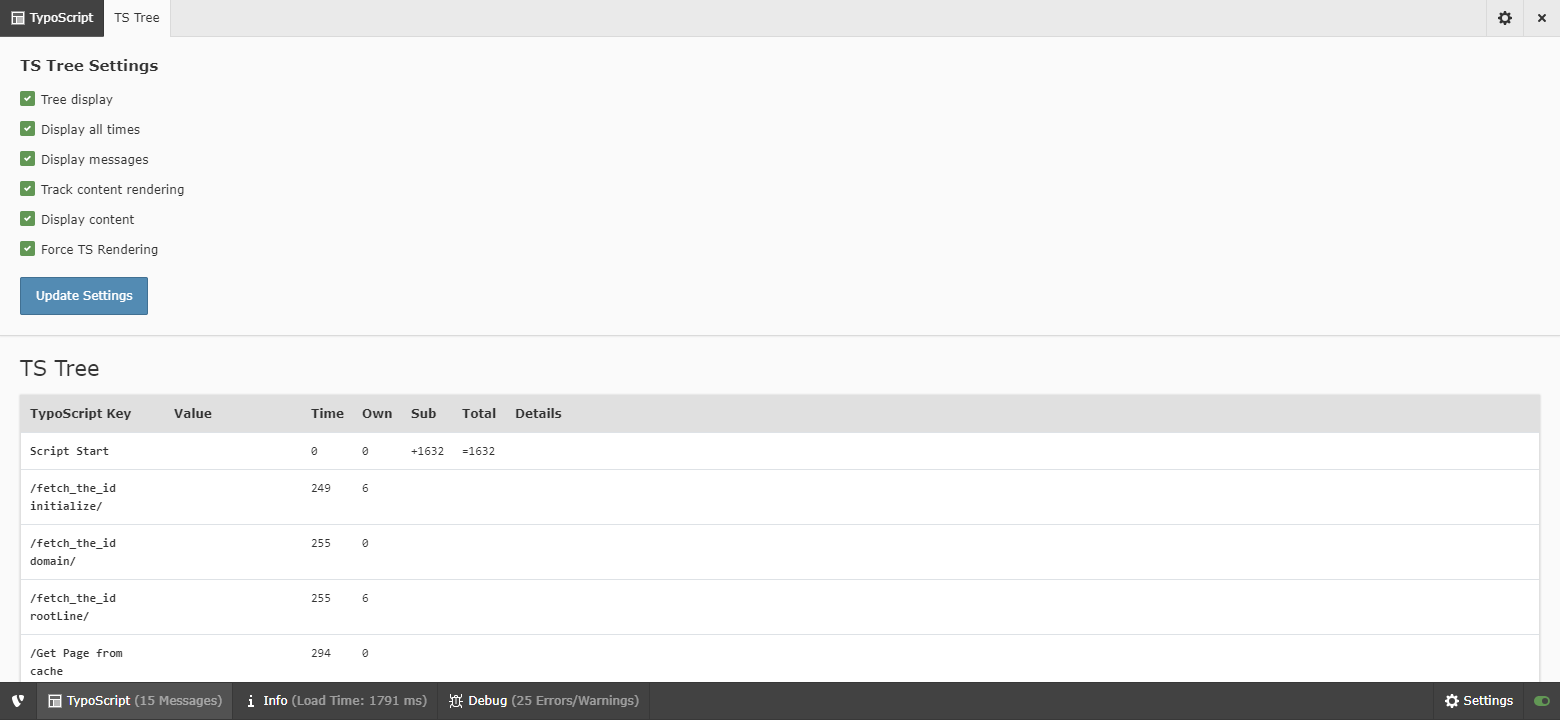
\includegraphics[width=0.90\linewidth]{BackendUserInterface/AdminPanelTypoScript.png}
	\end{figure}

\end{frame}

% ------------------------------------------------------------------------------
% Admin Panel (3)

\begin{frame}[fragile]
	\frametitle{Gebruikersinterface backend}
	\framesubtitle{Adminpaneel (3)}

	Schermvoorbeeld onder toont configuratieopties ("Instellingen").

	\begin{figure}
		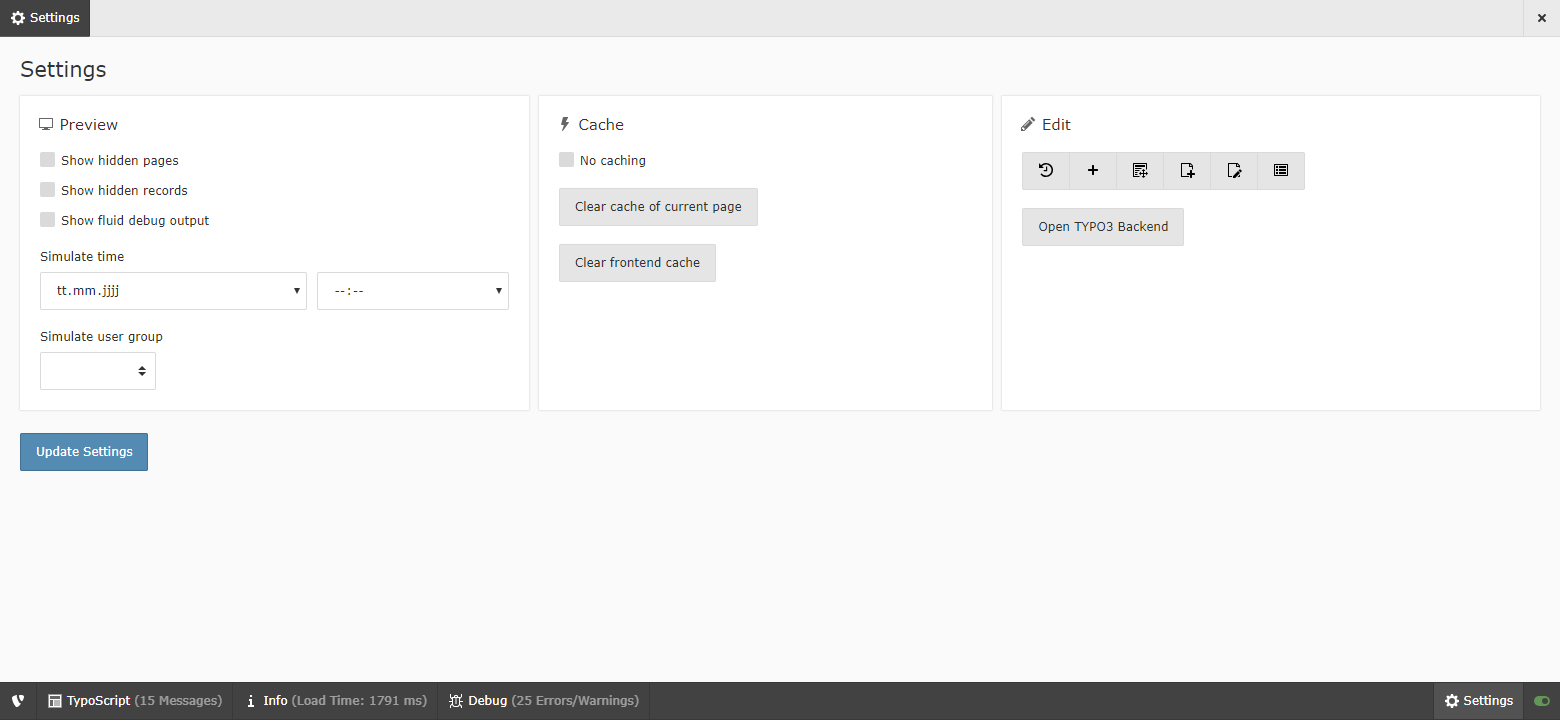
\includegraphics[width=0.90\linewidth]{BackendUserInterface/AdminPanelSettings.png}
	\end{figure}

\end{frame}

% ------------------------------------------------------------------------------
% #85398 - EXT:documentation removed

\begin{frame}[fragile]
	\frametitle{Gebruikersinterface backend}
	\framesubtitle{Extensie "Documentatie" verwijderd}

	Module "Documentatie" is verwijderd uit de TYPO3 backend.
    De module had technische en conceptuele problemen en acceptatie binnen de
    community was niet erg groot.
    \newline
    Alle documentatie blijft beschikbaar op \href{https://docs.typo3.org}{docs.typo3.org}.

	\begin{figure}
		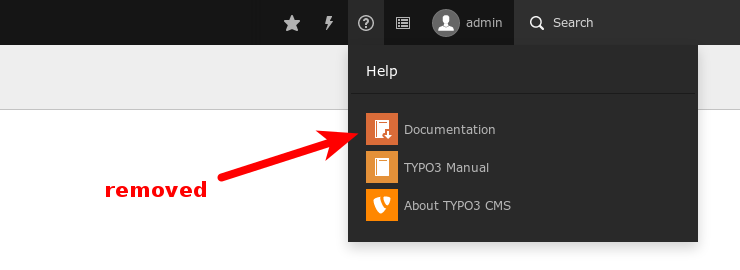
\includegraphics[width=0.70\linewidth]{BackendUserInterface/85398-ExtensionDocumentationRemoved.png}
	\end{figure}

\end{frame}

% ------------------------------------------------------------------------------
% #13265 - Select first element of page tree toolbar on initialization

\begin{frame}[fragile]
	\frametitle{Gebruikersinterface backend}
	\framesubtitle{Werkbalk paginaboom}

	Het eerste element van de werkbalk van de paginaboom wordt nu automatisch
	geselecteerd.

	\begin{figure}
		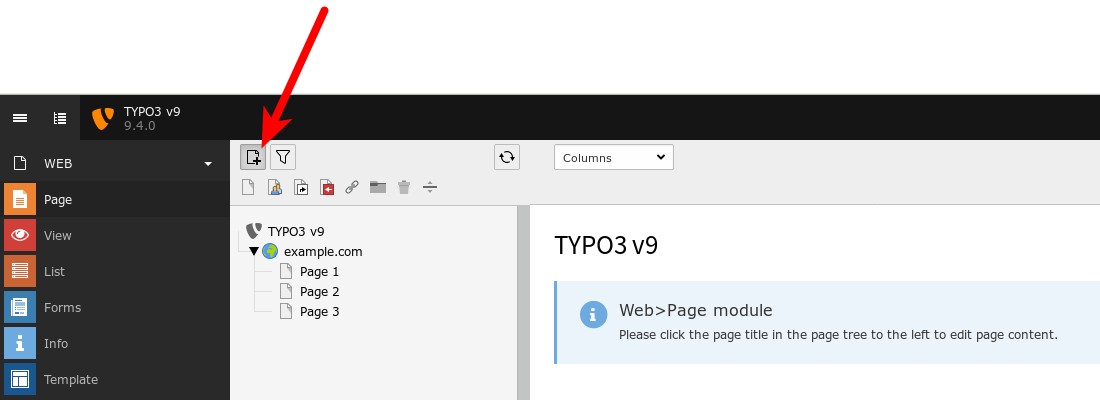
\includegraphics[width=0.90\linewidth]{BackendUserInterface/13265-FirstElementOfPageTree.png}
	\end{figure}

\end{frame}

% ------------------------------------------------------------------------------
% #85313 - Add notes field to pages table

\begin{frame}[fragile]
	\frametitle{Gebruikersinterface backend}
	\framesubtitle{Paginanotities}

	Pagina's hebben nu een veld "beschrijving" (tabblad "Notities") waarmee
	gebruikers notities kunnen toevoegen. Andere gebruikers kunnen ze inzien
	en bewerken.

	\begin{figure}
		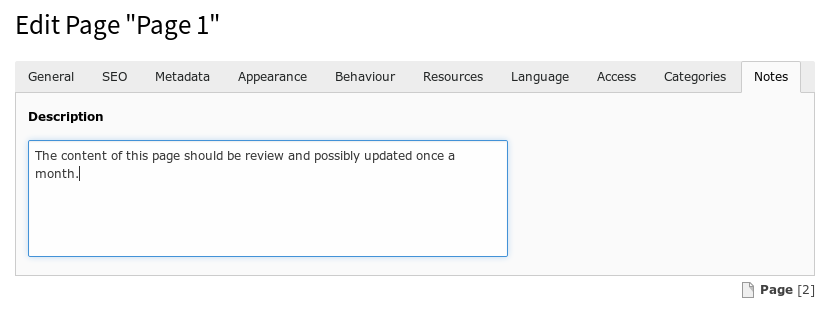
\includegraphics[width=0.90\linewidth]{BackendUserInterface/85313-NotesFieldForPages.png}
	\end{figure}

\end{frame}

% ------------------------------------------------------------------------------
% #xxxxx - Languages Visible in Frontend

\begin{frame}[fragile]
	\frametitle{Gebruikersinterface backend}
	\framesubtitle{Alleen gedefinieerde talen}

	Website talen in de backend zijn nu beperkt tot de talen gedefinieerd onder
	"Sitebeheer → Siteconfiguratie → Talen". Elke taal kan in- en uitgeschakeld
	worden.

	\begin{figure}
		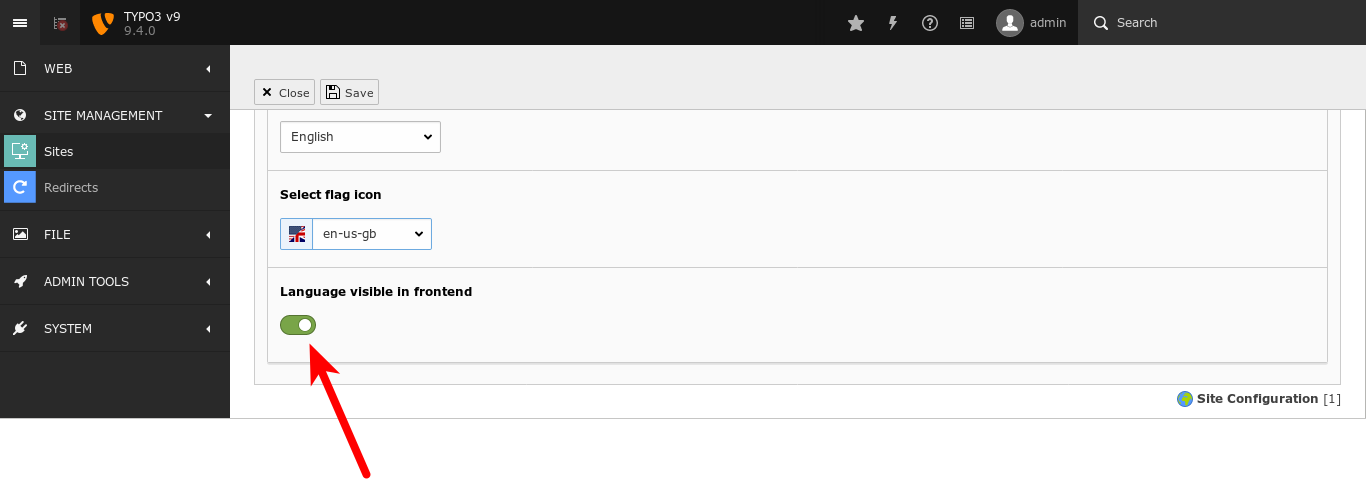
\includegraphics[width=0.90\linewidth]{BackendUserInterface/xxxxx-LanguagesVisibleInFrontend.png}
	\end{figure}

\end{frame}

% ------------------------------------------------------------------------------
% #85691 - Show page path in record info

\begin{frame}[fragile]
	\frametitle{Gebruikersinterface backend}
	\framesubtitle{Paginapad in record-informatie}

	Details over referenties naar een record bevatten nu het pad in de paginaboom.

	\begin{figure}
		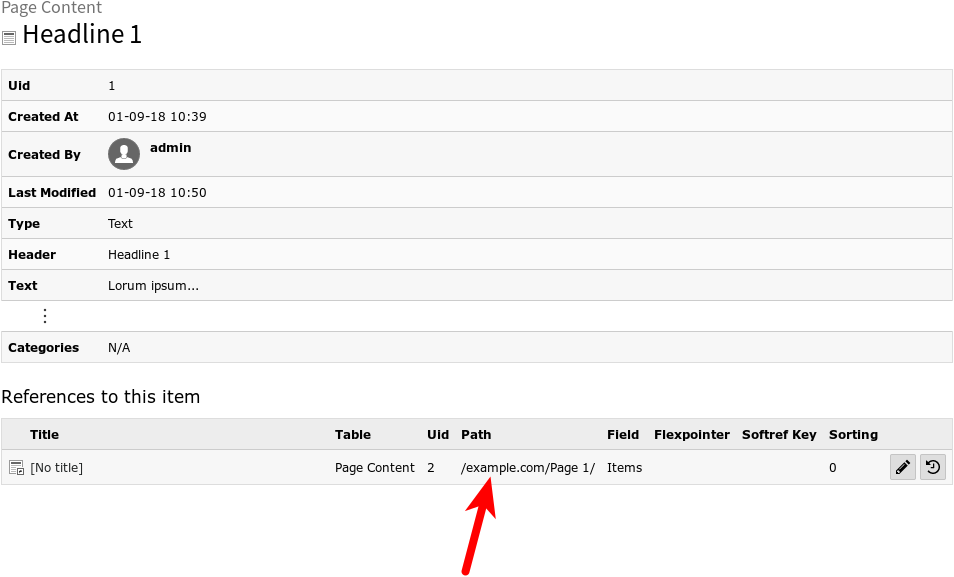
\includegraphics[width=0.70\linewidth]{BackendUserInterface/85691-ShowPagePathInRecordInfo.png}
	\end{figure}

\end{frame}

% ------------------------------------------------------------------------------
% Page-based URL Handling (aka "URL Routing")

\begin{frame}[fragile]
	\frametitle{Wijzigingen voor integrators}
	\framesubtitle{Paginagebaseerde URL-afhandeling}

 	TYPO3 ondersteunt nu standaard URL-afhandeling voor pagina's.

	\begin{figure}
		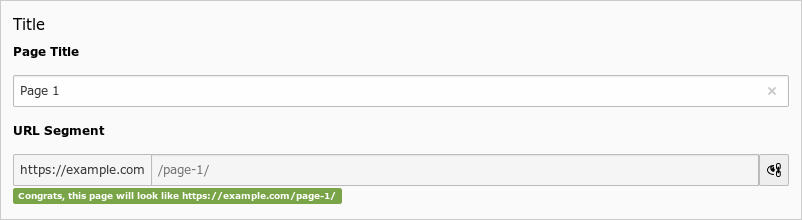
\includegraphics[width=0.90\linewidth]{BackendUserInterface/xxxxx-UrlRouting.png}
	\end{figure}

\end{frame}

% ------------------------------------------------------------------------------
% Modal Windows

% %%%%%%%%%%%%%%%%%%%%%%%%%%%%%%%%%%%%%%%%%%%%%%%%%%%%%%%%%%%%%% %
% Let's do not mention this in v9.4, but in v9.5 (TYPO3 v9 LTS). %
% We aim to achieve that all(!) popups use modal windows by the  %
% release of v9 LTS.                                             %
% %%%%%%%%%%%%%%%%%%%%%%%%%%%%%%%%%%%%%%%%%%%%%%%%%%%%%%%%%%%%%% %

%\begin{frame}[fragile]
%	\frametitle{Gebruikersinterface backend}
%	\framesubtitle{Modal Windows}
%
%	Almost all popup windows in the backend of TYPO3 are now "modal windows"
%	rather than small browser windows, which open.
%
%\end{frame}

% ------------------------------------------------------------------------------
